\chapter{Negocio}

\section{Introducción}
En esta capa se busca dar información acerca de una serie  de conceptos informativos para dar relevancia  en el dominio empresarial: un producto y contrato asociado, el significado de los objetos de negocio y el valor de los productos y servicios empresariales.\\
Para ello es necesario el diseño de 6 puntos de vista dentro de los cuales se encuentran: de organización, de cooperación de actor, de función de negocio, de proceso de negocio, de cooperación de proceso de negocio y de producto.\\
Los puntos de vista se mostrarán en dos partes, la primera de ellas será el modelo donde se encontrará una descripción del punto de vista acompañado de una tabla con la información de este y el meta-modelo correspondiente, en la segunda parte se encontrará el caso de estudio, es decir, el modelo donde será aplicado el meta-modelo previamente visto al proyecto y la organización en la que se está trabajando.
\newpage

\section{Punto de Vista de Organización}
\subsection{Descripción}
El punto de vista organizacional en la organización de la compañía, departamento, red de compañías, u otra identidad organizacional. Esto es posible para presentar modelos en este punto de vista como diagramas de bloques anidados, pero en el camino mas tradicional, tal como mapas organizacionales. El punto de vista organizacional es muy tratado en 	la identificación de competencias, autoridades y responsables en la organización.

\subsubsection{Metamodelo}
\begin{figure}[H]
	\centering
	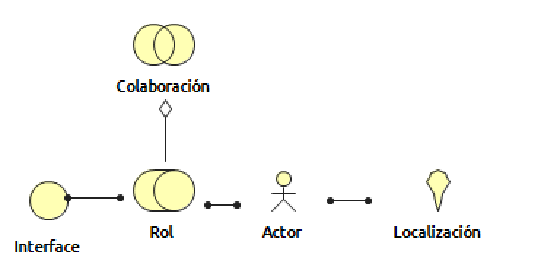
\includegraphics[width=1.0\textwidth]{imagenes/Metamodelos/Negocio/meta_organizacion.PDF}
	\caption{Metamodelo: Punto de Vista de Organización}
	\label{fig:gap_analysis}
\end{figure}

\subsubsection{Caso de Estudio}
En el siguiente punto de vista podemos resaltar la sucursal como localización principal de la organización; adicionalmente, se puede observar la participación de actores quienes son los pilares fundamentales para la realización de los principales procesos en la compañía. Estos son: Seguridad y Administración.

\begin{figure}[H]
	\centering
	\includegraphics[width=1.0\textwidth]{imagenes/Caso_estudio/Negocio/Organizacion.PDF}
	\caption{Caso de estudio: Punto de Vista de Organización}
	\label{fig:gap_analysis}
\end{figure}




\section{Punto de Vista de Cooperación de Actor}
\subsection{Descripción}
El punto de vista de Cooperación de actor se enfoca en las relaciones que se presentan entre un actor y su entorno, se puede decir que es un diagrama de contexto en el cual se coloca la organización en su entorno, además de esto se puede evidenciar clientes, proveedores y compañeros de negocio, tiene como objetivo determinar dependencias y colaboraciones externas y ver la relación con los actores que se encuentran en este diagrama, tenemos por otra parte que en este punto de vista se puede evidenciar el número de actores cooperantes  de negocio van a tener participación en esta capa o cuantos componentes de aplicación interactúan para formar un proceso de negocio.

\subsubsection{Metamodelo}
\begin{figure}[H]
	\centering
	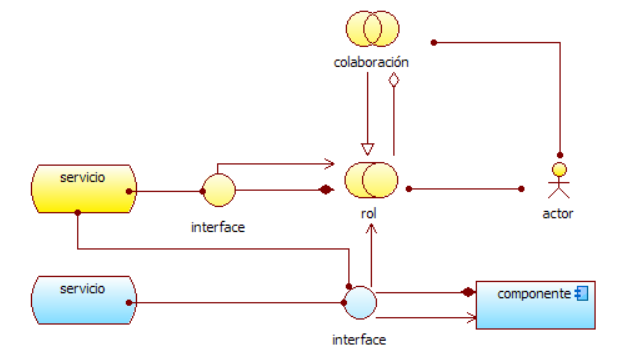
\includegraphics[width=1.0\textwidth]{imagenes/Metamodelos/Negocio/meta_cooperacion_actor.png}
	\caption{Metamodelo: Punto de Vista de Organización}
	\label{fig:gap_analysis}
\end{figure}




\subsubsection{Caso de Estudio}
La colaboración Espacio de Parqueadero, surge de la interacción de los roles Sucursal y Clientes del Parqueadero. Por parte de la sucursal, brindando el terrero de parqueo; y por parte de los clientes, al realizar el uso del mismo a través de la interface que se encuentra de cara a ellos, la Recepción.
\begin{figure}[H]
	\centering
	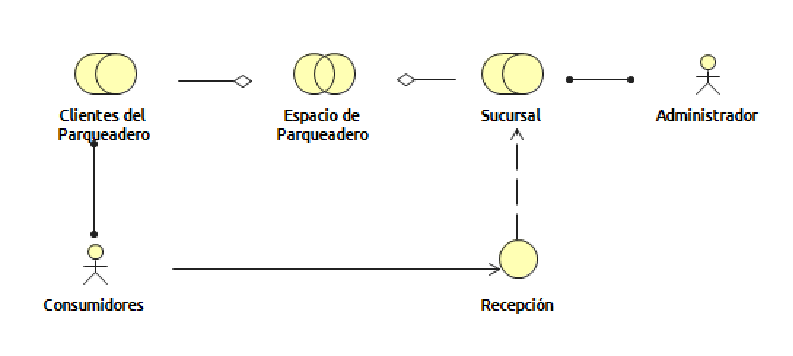
\includegraphics[width=1.0\textwidth]{imagenes/Caso_estudio/Negocio/CopActor.PDF}
	\caption{Caso de estudio: Punto de Vista de Cooperación de Actor}
	\label{fig:gap_analysis}
\end{figure}










\section{Punto de Vista de Función de Negocio}
\subsection{Descripción}
El punto de vista Función de negocio muestra las principales funciones de negocio de una organización y sus relaciones en términos de los flujos de información, valor o bienes entre ellos. Las funciones empresariales se utilizan para representar los aspectos más estables de una empresa en términos de las actividades primarias que realiza, independientemente de los cambios organizacionales o desarrollos tecnológicos.

Por lo tanto, la arquitectura de la función comercial de las empresas que operan en el mismo mercado a menudo muestran similitudes cercanas. Por lo tanto, el punto de vista de la función empresarial proporciona una visión de alto nivel de las operaciones generales de la empresa y puede utilizarse para identificar las competencias necesarias o estructurar una organización de acuerdo con sus principales actividades.


\subsubsection{Metamodelo}
\begin{figure}[H]
	\centering
	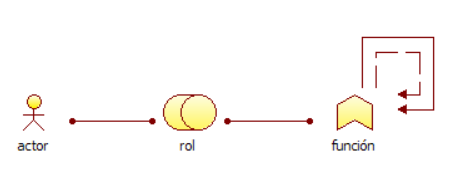
\includegraphics[width=1.0\textwidth]{imagenes/Metamodelos/Negocio/meta_funcion_negocio.png}
	\caption{Metamodelo: Punto de Vista de Función de Negocio}
	\label{fig:gap_analysis}
\end{figure}



\subsubsection{Caso de Estudio}
En el siguiente punto de vista se resalta la presencia de los actores Operario y Jefe de Seguridad, quienes llevan a cabo funciones específicas de los roles de Operación y Seguridad, tales como: Registro de Ingreso, Asignación de Parqueadero, Registro de Usuarios, Registro de Pagos, Registro de Retiros y Verificación de propiedad del vehículo.

\begin{figure}[H]
	\centering
	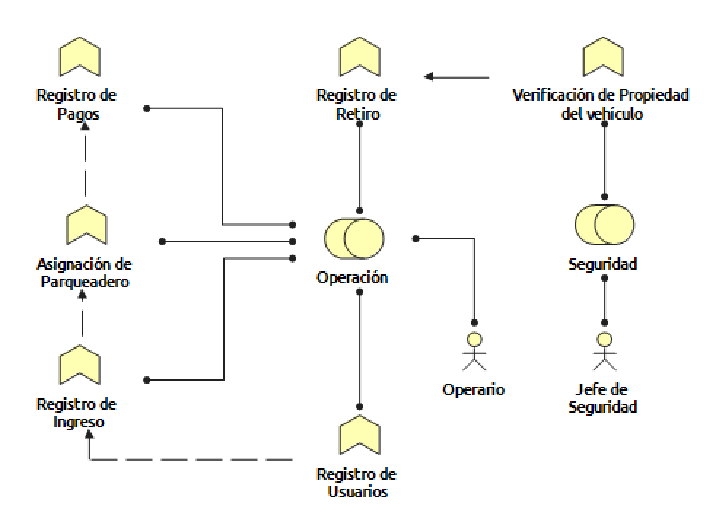
\includegraphics[width=1.0\textwidth]{imagenes/Caso_estudio/Negocio/FunNegocio.PDF}
	\caption{Caso de estudio: Punto de vista de función de negocio.}
	\label{fig:gap_analysis}
\end{figure}








\section{Punto de Vista de Proceso de Negocio}
\subsection{Descripción}
El punto de vista de proceso de negocio es usado para ver la estructura desde un nivel alto además de esto de poder evidenciar la composición de uno o más procesos de negocio, dentro de este punto de vista podemos resaltar que se enfoca en los servicios que un proceso de negocio puede ofrecer al cliente mostrando como este proceso puede contribuir para la realización de productos, por otro lado se puede hacer una asociación en cuanto a responsabilidades que tienen los actores asociados y los roles dentro de este proceso de negocio y por último en este punto de vista podemos evidenciar la información utilizada por el proceso de negocio.

\subsubsection{Metamodelo}
\begin{figure}[H]
	\centering
	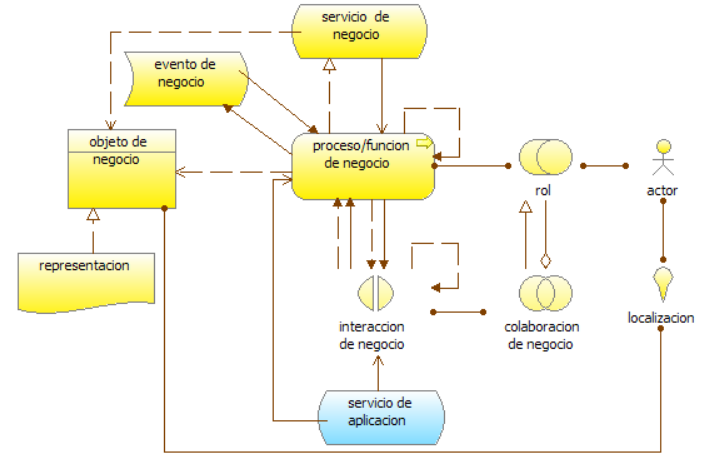
\includegraphics[width=1.0\textwidth]{imagenes/Metamodelos/Negocio/meta_proceso_negocio.png}
	\caption{Metamodelo: Punto de Vista de Proceso de Negocio}
	\label{fig:gap_analysis}
\end{figure}


\subsubsection{Caso de Estudio}
En este punto de vista podemos resaltar el proceso principal de la organización: Renta de espacio de parqueo, el cual es originado por una solicitud del espacio y finaliza en el retiro del vehículo. Dentro de este proceso tenemos los subprocesos de: Registro de Usuario, Registro de Ingreso, Asignación de Espacio, Vigilancia de Vehículo, Cálculo de tarifa y Registro de Pago.

\begin{figure}[H]
	\centering
	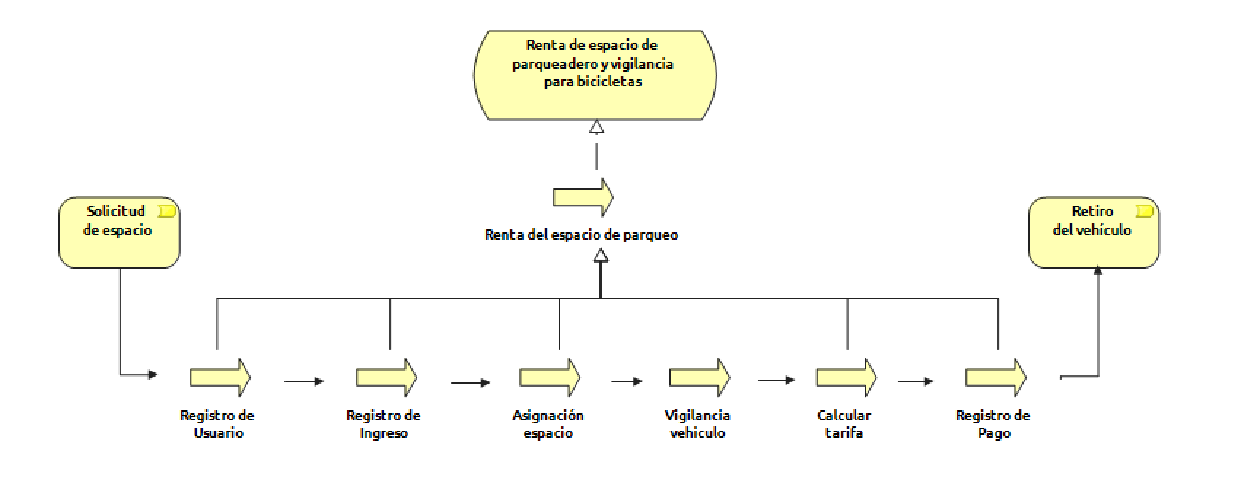
\includegraphics[width=1.0\textwidth]{imagenes/Caso_estudio/Negocio/ProNegocio.PDF}
	\caption{Caso de estudio: Punto de vista de proceso de negocio.}
	\label{fig:gap_analysis}
\end{figure}

\section{Punto de vista de Cooperación de procesos de negocio.}
\subsection{Descripción}
El punto de vista de Cooperación de Proceso de Negocio se utiliza para mostrar las relaciones de
uno o más procesos de negocio entre sí y / o con su entorno. Puede utilizarse tanto para crear un diseño
de alto nivel de procesos empresariales dentro de su contexto como para proporcionar un gestor
operativo responsable de uno o más de dichos procesos con información sobre sus dependencias

\subsubsection{Metamodelo}
\begin{figure}[H]
	\centering
	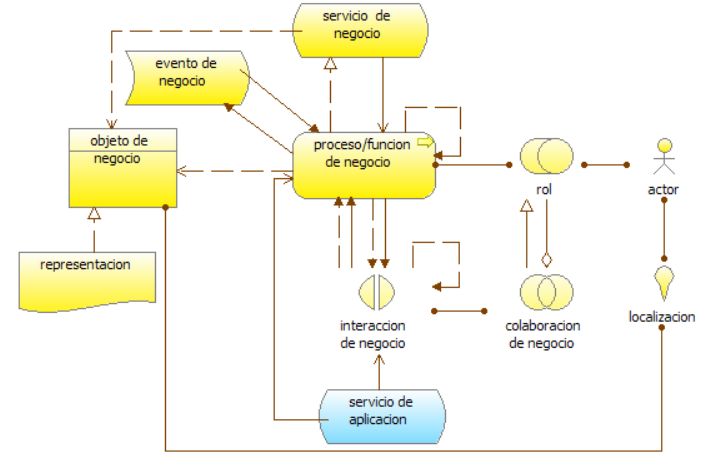
\includegraphics[width=1.0\textwidth]{imagenes/Metamodelos/Negocio/meta_cooperacion_proceso_negocio.png}
	\caption{Metamodelo: Punto de Vista de Cooperación de Negocio}
	\label{fig:gap_analysis}
\end{figure}



\subsubsection{Caso de Estudio}
Adicional al punto de vista anterior, se evidencian los roles involucrados, Administrador y Agente de Seguridad, en el proceso Renta de espacio de parqueo, para llevar a cabo el cumplimiento del servicio fundamental de la organización, Renta de espacio de parqueadero y vigilancia para bicicletas.

\begin{figure}[H]
	\centering
	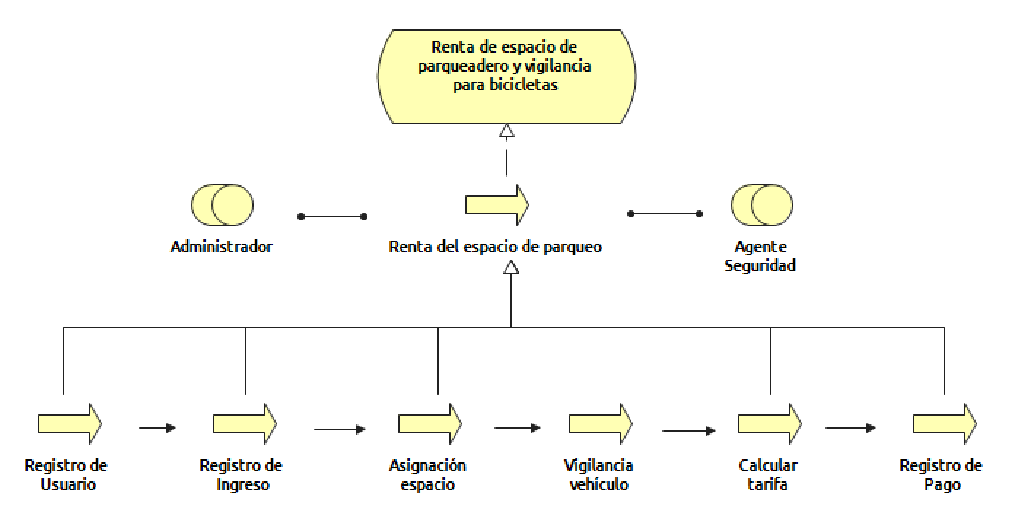
\includegraphics[width=1.0\textwidth]{imagenes/Caso_estudio/Negocio/CoProNegocios.PDF}
	\caption{Caso de estudio: Punto de vista de colabroacion de procesos de negocio.}
	\label{fig:gap_analysis}
\end{figure}


\section{Punto de Vista de Producto}

\subsection{Descripción}
El punto de vista del producto representa el valor que ese producto ofrece a los clientes u otros involucrados y muestra la composición de uno o mas productos en términos de los servicios constituidos y la asociación de contratos u otros acuerdos. Esto también puede ser usado para mostrar los canales de interfaces que este producto ofrece, y los eventos asociados con el producto. Un punto de vista del producto es típicamente usado en el desarrollo del producto a el diseño del producto por la composición de servicios existentes o la identificación que nuevos servicios tiene que ser creados para este producto,dando el valor a las expectativas del cliente para este. Este puede servir para la entrada para la arquitectura del proceso de negocio y otros que necesiten diseñar el proceso y ICT realizan estos productos. 

\subsubsection{Metamodelo}
\begin{figure}[H]
	\centering
	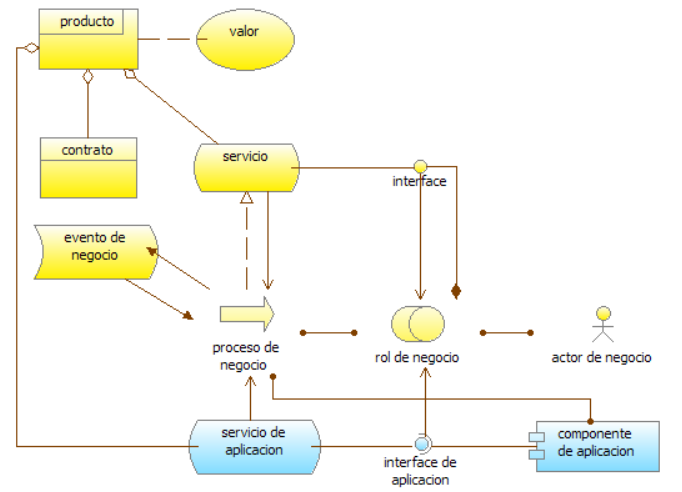
\includegraphics[width=1.0\textwidth]{imagenes/Metamodelos/Negocio/meta_producto.png}
	\caption{Metamodelo: Punto de Vista de Prodcuto}
	\label{fig:gap_analysis}
\end{figure}


\subsubsection{Caso de Estudio}
El producto principal que ofrece la organización, como se evidencia en los puntos de vista anteriores, es el espacio de parqueo, el cual se caracteriza por proponer espacios adecuados y seguros para las bicicletas de los clientes, a la vez de ofrecer un servicio integral de vigilancia permanente para los vehículos, soportados por sus correspondientes procesos.
\begin{figure}[H]
	\centering
	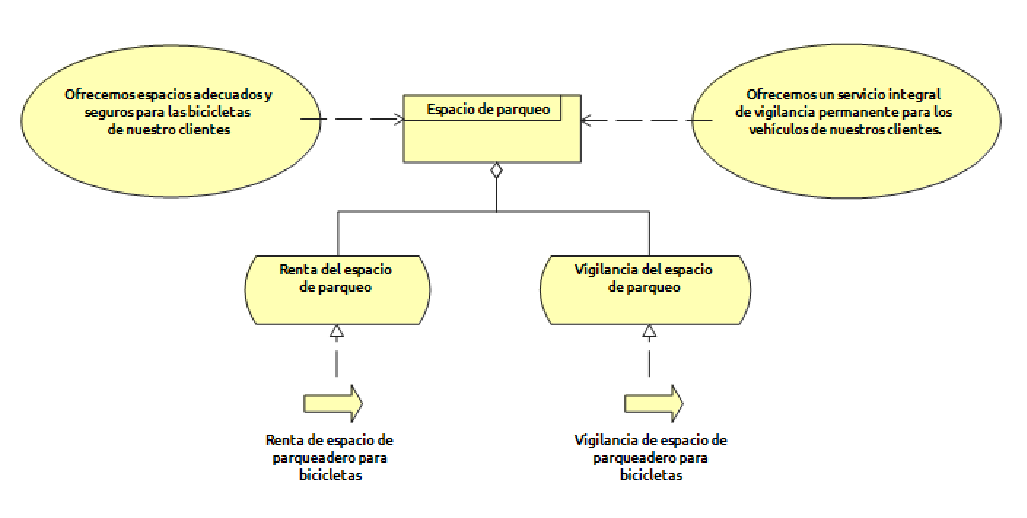
\includegraphics[width=1.0\textwidth]{imagenes/Caso_estudio/Negocio/Producto.PDF}
	\caption{Caso de estudio: Punto de vista de producto}
	\label{fig:gap_analysis}
\end{figure}


